\documentclass[12pt,a4paper]{beamer}
\usepackage[utf8x]{inputenc}
\usepackage{ucs}
\usepackage[english]{babel}
%\usepackage[german]{babel}
\usepackage{amsmath}
\usepackage{amsfonts}
\usepackage{amssymb}
\author{Michael Haas, haas@cl.uni-heidelberg.de}
\title{Rudolph \& Giesbrecht: Compositional Matrix-Space Models of Language}
\subtitle{Seminar: Distributionelle Semantik jenseits der Wortbedeutung (Matthias Hartung)}
\date{24-06-2013}
\newcommand{\tuple}[1]{\ensuremath{\left \langle #1 \right \rangle }}
\newcommand{\setof}[1]{\ensuremath{\left \{ #1 \right \}}}

\begin{document}


\begin{frame}
\maketitle
\end{frame}

\begin{frame}{Overview}
\begin{itemize}
%\item Previous approaches % incl problems
\item Idea \& Approach % incl motivation, or see prev?
\item Foundations
\begin{itemize}
    \item Plausibility % grounding in other theories
    \item Encoding VSM % + examples
    \item Encoding symbolic approaches
    \item Combination of different approaches
\end{itemize}
%\item Recap CMSM
\item A first implementation: Sentiment Analysis
\begin{itemize}
    \item Algorithm % cursory
    \item Results % cursory - was baseline sensible? what is state of the art?
\end{itemize}
\item Recap \& Discussion
\item \textbf{Questions? Too fast? Ask!}
\end{itemize}
\end{frame}

\begin{frame}{Idea \& Approach}
\begin{itemize}
\item Previous work on compositionality
    \begin{itemize}
    \item Operations between vectors, such as additions
    \item Tensor-Produkt between vectors, yielding matrices % resulting in n-dimensional matrices%
    \item Verbs as matrixes, nouns as vectors
\end{itemize}
\item Now: everything is a quadratic matrix, thus a linear mapping
\item Now: composition operation is matrix product
\end{itemize}
$\to$ VSM good enough for token meaning, but CMSM needed for composition
\end{frame}


\begin{frame}{Idea \& Approach}
\begin{itemize}
\item Mapping $[[\cdot]]$: maps tokens into semantical space $ \mathbb{S}=\mathbb{R}^{n \times n} $
\item Mapping chosen so that composition operation can be matrix multiplication 

\end{itemize}
\end{frame}


\begin{frame}{Foundations}
\begin{itemize}
\item \textbf{Plausibility in various systems}
\item CMSMs can represent various VSM
\item CMSMs can represent formal languages
\item Different representations can be combined
\end{itemize}
\end{frame}

\begin{frame}{Foundations: Plausibility: Algebraic Properties}
\begin{itemize}
\item Traditional VSM (e.g. Vector Mixture (Lapata, Mitchell, 2010??) 
 use associate and commutative operators
\end{itemize}
$\to$ Commutativity ignores word order
\begin{itemize}
\item Matrix multiplication is \textbf{non-commutative}
\end{itemize}
\end{frame}

\begin{frame}{Foundations: Plausibility: Neurological}
\begin{itemize}
\item Mental state: vector of neuron excitation values
\item Word as stimulus transforms mental state
\end{itemize}
$\to$ word is a function mapping mental states to mental states
\begin{itemize}
\item Arbitrary length transformations realised through matrix multiplication
\end{itemize}
\end{frame}

\begin{frame}{Foundations: Plausibility: Psychological}
\begin{itemize}
\item Working memory: represented by neural state vector %TODO: look up working memory - baddeley, 2003%
\item Matrices support memory operations: storage, deletion, copy
\end{itemize}
$to$ Anaphora resolution
\end{frame}

\begin{frame}{Foundations}
\begin{itemize}
\item Plausibility in various systems
\item \textbf{CMSMs can represent various VSM}
\item CMSMs can represent formal languages
\item Different representations can be combined
\end{itemize}
\end{frame}


\begin{frame}{Foundations: Vector Space Models}
CMSM encode Vector Space models
\begin{itemize}
\item Represent vector composition operation $\bowtie$ as matrix multiplication between mapped vectors
\item Map vectors into matrix space: $\psi_{\bowtie} \mathbb{R}^{n} \to \mathbb{R}^{n'\times n'} $
$$ v_{1} \bowtie \ldots \bowtie v_{k} = \psi_{\bowtie}^{-1}(\psi_{\bowtie}(v_{1}) \ldots \psi_{\bowtie}(v_{k}) )$$
\end{itemize}
\end{frame}


\begin{frame}{Foundations: VSM: Vector Addition}
\begin{itemize}
\item Basic model for semantic composition: composite meaning calculated by token addition $v_{w} = \sum_{i=1}^{k}v_{\sigma_{i}}$
% Where is the citation for that?
\item Map vectors into matrix space
$$  \psi_{+}(v_{\sigma}) =
\left( \begin{array}{ccc|c}
1 & \cdots & 0 & 0 \\
\vdots & \ddots & & \vdots \\
0 &  & 1 & 0 \\ \hline
&  v_{\sigma} & & 1 \end{array} \right) $$
\item So that $\psi_{+}^{-1} (\psi_{+}(v_{\sigma_{1}}) \ldots \psi_{+}(v_{\sigma_{k}})) = v_{\sigma_{1}} + \ldots + v_{\sigma_{k}}$
\end{itemize}
\end{frame}

\begin{frame}{Foundations: VSM: Vector Addition: Example}
\begin{itemize}
\item $w = v_{\sigma_{1}}v_{\sigma_{2}}$
\item $v_{\sigma_{1}} = (2,5)$, $v_{\sigma_{2}} = (3,1)$
\item Plug into $v_{w} = \sum_{i=1}^{k}v_{\sigma_{i}}$
\item $v_{w} = (2,5)+(3,1) = (5,6)$
\item $\psi_{+}(v_{1}) = \left( \begin{array}{cc|c}
1 & 0 & 0 \\
0 & 1 & 0 \\
2 & 5 & 1 \end{array} \right) $
\item  $\psi_{+}(v_{2}) = \left( \begin{array}{cc|c}
1 & 0 & 0 \\
0 & 1 & 0 \\
3 & 1 & 1 \end{array} \right) $
\end{itemize}
\end{frame}


\begin{frame}{Foundations: VSM: Vector Addition: Example}
\begin{itemize}
\item $v_{\sigma_{1}} = (2,5)$, $v_{\sigma_{2}} = (3,1)$
\item $\psi_{+}(v_{\sigma_{1}}) = \left( \begin{array}{cc|c}
1 & 0 & 0 \\
0 & 1 & 0 \\
2 & 5 & 1 \end{array} \right) $
\item  $\psi_{+}(v_{\sigma_{2}}) = \left( \begin{array}{cc|c}
1 & 0 & 0 \\
0 & 1 & 0 \\
3 & 1 & 1 \end{array} \right) $

$$ \psi_{+}(v_{\sigma_{1}}) \psi_{+}(v_{\sigma_{2}}) = 
\left( \begin{array}{cc|c}
1 & 0 & 0 \\
0 & 1 & 0 \\
5 & 6 & 1 \end{array} \right)
$$
% 5 = A_31 * B_11 + A_32 + B_21 (=0)  +  A_33*B_31
% 6 = A_31 * B_12 (= 0) + A_32 * B_22 + A_33 * B_33
\end{itemize}
\end{frame}

\begin{frame}{Foundations: VSM: Component-Wise Multiplication}
\begin{itemize}
\item CMSM can simulate Hadamard product
% Where is the citation here?
\item Hadamard product: component-wise multiplication
\item Hadamard product $\neq$ cross-product
\item $(A \bullet B)_{ij} = A_{ij} * B_{ij}$
\item Use different encoding function for vectors!
$$  \psi_{\bullet}(v_{\sigma}) =
\left( \begin{array}{cccc}
v_{\sigma}(1) & 0 & 0 & 0 \\
0 & v_{\sigma}(2) & 0 & 0 \\
0 & 0 & \ddots & 0 \\
0 & 0 & 0 & v_{\sigma}(n) \end{array} \right) $$

\item So that $\psi_{+}^{-1} (\psi_{+}(v_{\sigma_{1}}) \ldots \psi_{+}(v_{\sigma_{k}})) = v_{\sigma_{1}} \bullet \ldots \bullet v_{\sigma_{k}}$


\end{itemize}
\end{frame}




\begin{frame}{Foundations: VSM: Circular Convolution Product}
\begin{itemize}
\item CMSM can simulate Circular Convolution Product 
\item $v_{3}(i+1) = \sum_{k=0}^{n-1}{v_{1} (k+1) * v_{2} ( (i-k \bmod{n}) +1) }$
\item Encoding function:
$$  M(i,j) = v ((j - i \bmod{n} ) +1) $$
\item Encoded matrix:

$$\psi_{ \circledast } ( v(1), v(2), v(3) ) =
\left( \begin{array}{ccc}
v(1) & v(2) & v(3)  \\
v(3) & v(1) & v(2)  \\
v(2) & v(3) & v(1)  \end{array} \right)
$$

\item So that $\psi_{+}^{-1} (\psi_{+}(v_{\sigma_{1}}) \ldots \psi_{+}(v_{\sigma_{k}})) = v_{\sigma_{1}} \circledast \ldots \circledast v_{\sigma_{k}}$

\end{itemize}
\end{frame}


%\begin{frame}{Foundations: VSM: Permutation-based Approaches}
%\begin{itemize}
%\item Sahlgren et al 
%\end{itemize}
%\end{frame}

%\begin{frame}{Foundations: Symbolic Approaches: Group Theory}
%\begin{itemize}
%\item
%\end{itemize}
%\end{frame}


\begin{frame}{Foundations}
\begin{itemize}
\item Plausibility in various systems
\item CMSMs can represent various VSM
\item \textbf{CMSMs can represent formal languages}
\item Different representations can be combined
\end{itemize}
\end{frame}


\begin{frame}{Foundations: Symbolic Approaches: Regular Language}
\begin{itemize}
\item CMSM can simulate regular languages
\item Build transition matrices for finite state automaton
\item For every input token $\sigma$ build $[[\sigma]] = M$ with
$$ M(i,j) = \left\{\begin{array}{cl} 1, & \mbox{if } (q_{i},\sigma,q_{j}) \in \Delta) \\ 0, & \mbox{otherwise} \end{array}\right.  $$
\end{itemize}
\end{frame}


\begin{frame}{Foundations: Symbolic Approaches: Regular Language}
\begin{itemize}
\item Words: $w = \sigma_{1} \ldots \sigma{k} \in \Sigma^{*}$ 
\item Represents words as state transition matrix:
$$ M_{w} = [[\sigma_{1}]]\ldots [[\sigma_{k}]]  $$
\item Start and end state vectors:
$$ v_{I}(i) = \left\{\begin{array}{cl} 1, & \mbox{if } q_{i} \in Q_{I} \\ 0, & \mbox{otherwise} \end{array}\right. $$ 
$$ v_{F}(i) = \left\{\begin{array}{cl} 1, & \mbox{if } q_{i} \in Q_{F}) \\ 0, & \mbox{otherwise} \end{array}\right. $$
\item Word is accepted if
$$ v_{I}M_{w}v_{F}^{T} \ge 1 $$
\end{itemize}
\end{frame}



\begin{frame}{Foundations: Symbolic Approaches: Matrix Grammars}
\begin{itemize}
\item Matrix grammar $M := \tuple{[[\mathord{\cdot}]], AC}$
\item $[[\mathord{\cdot}]]$: mapping from $\Sigma$ to $n \times n $ matrix
\item $AC$: Acceptance conditions $ \setof{ \tuple{v'_{1}, v_{1}, r_{1}}, \ldots, \tuple{v'_{m}, v_{m}, r_{m}} }$
\item $v'_{1}, v_{1},\ldots,v'_{m}, v_{m} \in \mathbb{R}^{n}$
\item $r_{1}, \ldots, r_{2} \in \mathbb{R}$
\end{itemize}
\end{frame}

\begin{frame}{Foundations: Symbolic Approaches: Matrix Grammars: Acceptance}
\begin{itemize}
\item $AC$: Acceptance conditions $ \setof{ \tuple{v'_{1}, v_{1}, r_{1}}, \ldots, \tuple{v'_{m}, v_{m}, r_{m}} }$
\item Word $\sigma_{1},\ldots,\sigma{k}$ in $L(M)$ if for all $i \in [1,\ldots,m]$ 
$$v'_{i}[[\sigma_{1}]] \ldots [[\sigma_{k}]] v_{i}^{'T} \ge r_{i}$$
\end{itemize}
\end{frame}


\begin{frame}{Foundations: Symbolic Approaches: Matrix Grammars: Properties}
\begin{itemize}
\item Matricible languages
\begin{itemize}
    \item palindrome language
    \item $\setof{ a^{m} b ^{m} c^{m}  }$ (non-context-free)
\end{itemize}
\item All languages characterized by set of linear equations on letter count
\item Intersection of matricible language
\item But: (likely) not all context-free languages matricible
\end{itemize}
\end{frame}



\begin{frame}{Foundations}
\begin{itemize}
\item Plausibility in various systems
\item CMSMs can represent various VSM
\item CMSMs can represent formal languages
\item \textbf{Different representations can be combined}
\end{itemize}
\end{frame}


\begin{frame}{Foundations: Combination of different approaches}
\begin{itemize}
\item Combine two models by combining their mapping matrices
\item First model $[[\sigma_{1}]]$, second model $([\sigma_{1}])$
\end{itemize}

$$  \{[\sigma_{i}]\} =
\left( \begin{array}{cccc|cccc}
 &  &  &  & 0 & 0 & 0 & 0   \\
 &  &  &  & 0 & 0 & 0 & 0   \\
 & [[\sigma_{1}]]  &  &  & 0 & 0 & 0 & 0   \\
 &  &  &  & 0 & 0 & 0 & 0   \\ \hline
0 & 0 & 0 & 0 &  &  &  &    \\
0 & 0 & 0 & 0 &  &  &  &    \\
0 & 0 & 0 & 0 &  &  & ([\sigma_{1}])  &    \\
0 & 0 & 0 & 0 &  &  &  &    \\
\end{array} \right) $$


\end{frame}


\begin{frame}{Recap CMSM}
\begin{itemize}
\item Matrix-based model of compositionality
\item Algebraic, neurological and psychological plausbility
\item Very expressive
\item But: how to obtain CMSMs?
\item But: how well does model actually perform?
\end{itemize}

\end{frame}


\begin{frame}{Overview}
\begin{itemize}
%\item Previous approaches % incl problems
\item Idea \& Approach % incl motivation, or see prev?
\item Foundations
\begin{itemize}
    \item Plausibility % grounding in other theories
    \item Encoding VSM % + examples
    \item Encoding symbolic approaches
    \item Combination of different approaches
\end{itemize}
%\item Recap CMSM
\item \textbf{A first implementation: Sentiment Analysis}
\begin{itemize}
    \item Algorithm % cursory
    \item Results % cursory - was baseline sensible? what is state of the art?
\end{itemize}
\item Recap \& Discussion
\end{itemize}
\end{frame}



\begin{frame}{CMSM for Sentiment Analysis}
\begin{itemize}
\item A first implementation proposed by Yessenalina \&  Cardie (2011)
%\item Combine adverb "very" with positive polar adjective "good"
\item "very good" $\to$ increased positive polarity
\item "not good", "not perfect" $\to$ dampening
\item "prevent cancer"
\item Typical approaches: bag-of-words
\end{itemize}
\end{frame}


\begin{frame}{CMSM for Sentiment Analysis: Idea}
\begin{itemize}
\item "very good"
\item Typical approaches: bag-of-words
\item Here: Model  words as matrices
\item Combine word matrices using matrix multiplication
\end{itemize}
\end{frame}

\begin{frame}{CMSM for Sentiment Analysis: Approach}
\begin{itemize}
\item Sentiment represented on five-point ordinal scale
\item Ordered Logistic Regression framework
\item Baseline: bag-of-words
\begin{itemize}
    \item OLogReg model learns one weight per word
\end{itemize}
\item Bag-of-words OLogReg is convex, therefore we will find global optimum
\item Matrix-Space OLogReg is non-convex, needs good initialisation
\item Initizalize Matrix-Space OLogReg with result of bag-of-words OLogReg
 
\end{itemize}
\end{frame}


\begin{frame}{CMSM for Sentiment Analysis: Eval}
\begin{itemize}
\item Evaluation data: Multi-Perspective Question Answering corpus \footnote{MPQA, Wiebe et al, 2005}
\item 535 newswire documents annotated with phrase-level subjectivity and intensity
\item Training: 10-fold cross validation on 8022 lemmatized phrases
\item Methods:
\begin{itemize}
    \item PRank
    \item Bag-of-words OLogReg
    \item Matrix-Space OLogReg+RandInit
    \item Matrix-Space OLogReg+BowInit
\end{itemize}
\end{itemize}
\end{frame}


\begin{frame}{CMSM for Sentiment Analysis: Methods}
\begin{itemize}
\item PRank
\item Bag-of-words OLogReg
\item Matrix-Space OLogReg+RandInit
\item Matrix-Space OLogReg+BowInit
\end{itemize}
\end{frame}



\begin{frame}{CMSM for Sentiment Analysis: Eval Results}

\begin{figure}
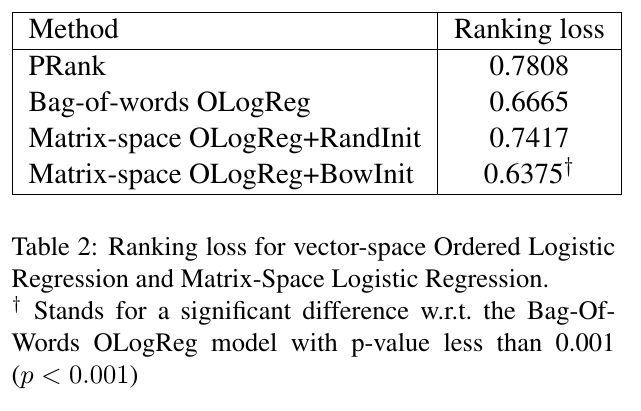
\includegraphics[width=\textwidth]{cmsm_for_se_table2.png}
\caption{Yessenalina \&  Cardie (2011)}
\end{figure}
\end{frame}


\begin{frame}{CMSM for Sentiment Analysis: Eval Results}
\begin{figure}
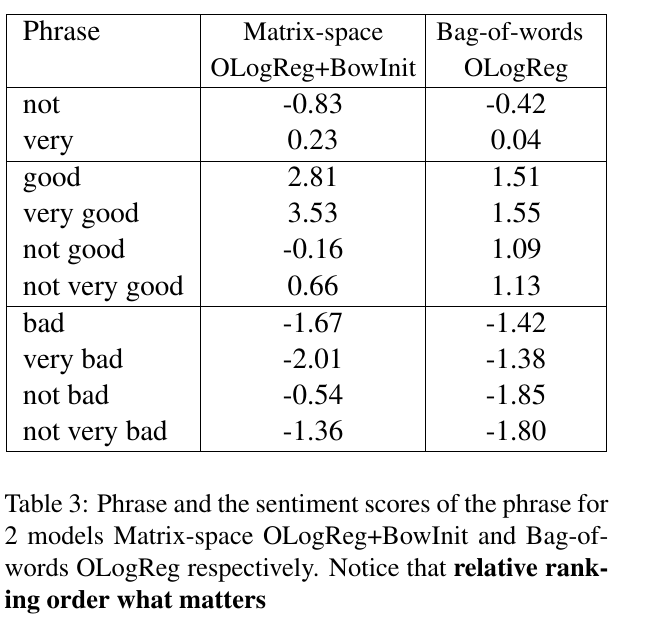
\includegraphics[scale=0.45]{cmsm_for_se_table3.png}
\caption{Yessenalina \&  Cardie (2011)}
\end{figure}

\end{frame}


\begin{frame}{Recap}
\begin{itemize}
\item Matrix-based model of compositionality
\item Algebraic, neurological and psychological plausbility
\item Very expressive
\item First implementation available
    \begin{itemize}
    \item Non-Convex learning scheme
    \end{itemize}
\end{itemize}
\end{frame}

\begin{frame}{Discussion}
\begin{itemize}
\item Is non-convex learning scheme viable?
\item Is performance of first implementation convincing?
\item Composition order? Negation scope? \cite{cmsmse} 
\item What about vector-matrix \textbf{multiplication}?
\item Sentiment Analysis: what is state of the art for specific task?
\end{itemize}
\end{frame}


\begin{frame}[allowframebreaks]{References}
\begin{thebibliography}{-}
% APA
\bibitem{cmsm} Rudolph, S., \& Giesbrecht, E. (2010, July). Compositional matrix-space models of language. In Proceedings of the 48th Annual Meeting of the Association for Computational Linguistics (pp. 907-916). Association for Computational Linguistics.
\bibitem{cmsmse} Yessenalina, A., \& Cardie, C. (2011, July). Compositional matrix-space models for sentiment analysis. In Proceedings of the Conference on Empirical Methods in Natural Language Processing (pp. 172-182). Association for Computational Linguistics.
\end{thebibliography}
\end{frame}
\end{document}

